\documentclass[
portrait,
% landscape,
a0paper%,
%draft
]
{baposter}
%
% load packages
% already loaded some useful packages for figures, tables and layout
% not all are needed to run this minimal example
\usepackage{graphicx}
\usepackage[percent]{overpic}
\usepackage[detect-weight]{siunitx}
\usepackage{tabto}
\usepackage{booktabs}
\usepackage{amsmath}
\usepackage{float}
\usepackage{multirow}
\usepackage[hyphens]{url}
\usepackage{enumitem}
\usepackage{ragged2e}
\usepackage{qrcode}
\usepackage{acro}
% add additional packages you need here
%
% for now usig bibitem, but if you want ...
%\usepackage[backend=biber]{biblatex} 
%
% customizing 
\newlength{\mytextsize}
\newcommand\e{\cdot 10^}
\setlength{\unitlength}{1.0cm}
%
% define cern blue  
% \definecolor{maincolor}{RGB}{80,110,185}
\definecolor{maincolor}{RGB}{60,80,135}
% \definecolor{maincolor}{RGB}{210,50,70}
% \definecolor{maincolor}{RGB}{163,107,115}
% \definecolor{maincolor}{RGB}{175,93,50}
% \definecolor{maincolor}{RGB}{125,200,200}
% \definecolor{headercolor}{RGB}{0,0,0}
\definecolor{headercolor}{RGB}{255,255,255}
\def\highlightcolorOne{blue!60!cyan!03}
\def\highlightcolorTwo{blue!60!cyan!15}
\definecolor{highlightcolor}{RGB}{70,150,255}
% fonts
\usepackage[scaled]{helvet}
% \renewcommand*\familydefault{\sfdefault}
%
%

%%% This file contains definitions of various useful macros and environments %%%
%%% Please add more macros here instead of cluttering other files with them. %%%

%%% Minor tweaks of style

% These macros employ a little dirty trick to convince LaTeX to typeset
% chapter headings sanely, without lots of empty space above them.
% Feel free to ignore.
\makeatletter
\def\@makechapterhead#1{
  {\parindent \z@ \raggedright \normalfont
   \Huge\bfseries \thechapter. #1
   \par\nobreak
   \vskip 20\p@
}}
\def\@makeschapterhead#1{
  {\parindent \z@ \raggedright \normalfont
   \Huge\bfseries #1
   \par\nobreak
   \vskip 20\p@
}}
\makeatother

% This macro defines a chapter, which is not numbered, but is included
% in the table of contents.
\def\chapwithtoc#1{
\chapter*{#1}
\addcontentsline{toc}{chapter}{#1}
}

% Draw black "slugs" whenever a line overflows, so that we can spot it easily.
\overfullrule=1mm

%%% Macros for definitions, theorems, claims, examples, ... (requires amsthm package)

\theoremstyle{plain}
\newtheorem{thm}{Theorem}
\newtheorem{lemma}[thm]{Lemma}
\newtheorem{claim}[thm]{Claim}

\theoremstyle{plain}
\newtheorem{defn}{Definition}
\newtheorem*{defn*}{Definition}

\theoremstyle{remark}
\newtheorem*{cor}{Corollary}
\newtheorem*{rem}{Remark}
\newtheorem*{example}{Example}

%%% An environment for proofs

\newenvironment{myproof}{
  \par\medskip\noindent
  \textit{Proof}.
}{
\newline
\rightline{$\qedsymbol$}
}

%%% An environment for typesetting of program code and input/output
%%% of programs. (Requires the fancyvrb package -- fancy verbatim.)

\DefineVerbatimEnvironment{code}{Verbatim}{fontsize=\small, frame=single}

%%% The field of all real and natural numbers
\newcommand{\R}{\mathbb{R}}
\newcommand{\N}{\mathbb{N}}

%%% Useful operators for statistics and probability
\DeclareMathOperator{\pr}{\textsf{P}}
\DeclareMathOperator{\E}{\textsf{E}\,}
\DeclareMathOperator{\var}{\textrm{var}}
\DeclareMathOperator{\sd}{\textrm{sd}}

%%% Transposition of a vector/matrix
\newcommand{\T}[1]{#1^\top}

%%% Various math goodies
\newcommand{\goto}{\rightarrow}
\newcommand{\gotop}{\stackrel{P}{\longrightarrow}}
\newcommand{\maon}[1]{o(n^{#1})}
\newcommand{\abs}[1]{\left|{#1}\right|}
\newcommand{\dint}{\int_0^\tau\!\!\int_0^\tau}
\newcommand{\isqr}[1]{\frac{1}{\sqrt{#1}}}

%%% Various table goodies
\newcommand{\pulrad}[1]{\raisebox{1.5ex}[0pt]{#1}}
\newcommand{\mc}[1]{\multicolumn{1}{c}{#1}}

%%% My macros ~~~~~~~~~~~~~~~~~~~~~~~~~~~~~~~~~~~~~~~~~~~~~~~~~~~~~~~~~~~~~~~~~~~~~~~~~~~~~~~~~~~~~~~~~~~~~~~

%%% Work-In-Progress designators --------------------------------------------------------
\newcommand{\todo}[1]{%
    \textcolor{orange}{\textbf{#1}}% Bold and orange text
    \marginpar{\textcolor{orange}{\PencilLeft}}% Symbol on the side of the page
    \PackageWarning{TODO}{#1}% Warning in LaTeX log
}
\newcommand{\toask}[1]{%
    \textcolor{blue}{\textbf{#1}}% Bold and orange text
    \marginpar{\textcolor{blue}{\large{\textbf{?}}}}% Symbol on the side of the page
    \PackageWarning{TODO}{#1}% Warning in LaTeX log
}
\newcommand{\wording}[1]{%
    \textcolor{brown}{#1}% orange text
    \marginpar{\textcolor{brown}{\PencilLeft}}% Symbol on the side of the page
}

%%% Typography or something -------------------------------------------------------------
% This macro defines a section, which is not numbered, but is included in the table of contents.
\def\secwithtoc#1{
\section*{#1}
\addcontentsline{toc}{section}{#1}
}

\newcommand{\tablenote}[2]{\multicolumn{#1}{p{0.95\textwidth}}{\footnotesize \emph{Note:} #2}}

%%% Math --------------------------------------------------------------------------------
\newcommand{\precedence}[2]{#1 \hspace{-0.2em} \rightarrow \hspace{-0.2em} #2}
\newcommand{\Jobs}{\mathcal{J}}
\newcommand{\Precedences}{\mathcal{P}}
\newcommand{\Orders}{\mathcal{O}}
\newcommand{\Resources}{\mathcal{R}}
\newcommand{\horizon}{T}

\newcommand{\duration}[1]{p_{#1}}
\newcommand{\deadline}[1]{\overset{\sim}{d}_{#1}} % TODO overset
\newcommand{\tardinessweight}[1]{w_{#1}}
\newcommand{\maxcapacity}[1]{R_{#1}}
\newcommand{\capacity}[2]{R^{(#2)}_{#1}}
\newcommand{\consumption}[2]{r_{#1 #2}}

\newcommand{\jobstart}[1]{S_{#1}}
\newcommand{\Schedule}{S}
\newcommand{\jobend}[1]{C_{#1}}
\newcommand{\Completions}{C}
\newcommand{\tardiness}[1]{T_{#1}}

\newcommand{\solutionOptimal}{S}
\newcommand{\solutionImproved}{S^*}
\newcommand{\OrdersSelected}{O^*}
\newcommand{\tardinessImproved}[1]{\tardiness{#1}^*}

\newcommand{\diff}[2]{\operatorname{diff}\hspace{-0.2em}\left( #1 ,\; #2 \right)}
\newcommand{\defeq}{\overset{\text{def}}{=}}

%%% Indicators -------------------------------------------------------
\newcommand{\indicator}[2]{\operatorname{#1}_{#2}}

\newcommand{\indMW}[1]{\indicator{MW}{#1}}
\newcommand{\indMUR}[1]{\indicator{MUR}{#1}}
\newcommand{\indAUAD}[1]{\indicator{AUAD}{#1}}
\newcommand{\indMRW}[1]{\indicator{MRW}{#1}}
\newcommand{\indMRUR}[1]{\indicator{MRUR}{#1}}
\newcommand{\indAUAC}[1]{\indicator{AUAC}{#1}}

% first  \ac{...}
% second \ac{...}
% long   \acl{...}
% short  \acs{...}
% full   \acf{...}
% Capitalize first letter of command to capitalize acronym


\DeclareAcronym{aps}{
    short=APS,
    long=Advanced Planning and Scheduling,
}

\DeclareAcronym{rcpsp}{
    short=RCPSP,
    long=Resource-Constrained Project Scheduling Problem
}

\DeclareAcronym{ebm}{
    short=EBM,
    long=Execution Bottleneck Machine
}

% Metrics
\DeclareAcronym{mw}{
    short=MW,
    long=Machine Workload
}
\DeclareAcronym{mur}{
    short=MUR,
    long=Machine Utilization Rate
}
\DeclareAcronym{auad}{
    short=AUAD,
    long=Average Uninterrupted Active Duration
}

\DeclareAcronym{mrw}{
    short=MRW,
    long=Machine Resource Workload
}
\DeclareAcronym{mrur}{
    short=MRUR,
    long=Machine Resource Utilization Rate
}
\DeclareAcronym{auac}{
    short=AUAC,
    long=Average Uninterrupted Active Consumption
}

\newcommand{\todo}[1]{%
    \textcolor{red}{\textbf{#1}}% Bold and red text
    \PackageWarning{TODO}{#1}% Warning in LaTeX log
}
% Custom headerbox command to left-align text
\newcommand{\leftalignedheaderbox}[3]{%
  \headerbox{#1}{#2}{%
  % \RaggedRight{%
  #3
% }
}}
\newcommand{\highlight}[1]{%
\textbf{\color{highlightcolor}#1}%
}

%##################################################################################
\begin{document}
%##################################################################################
\begin{poster}
{
  % options
  grid=false,%true,
  background=plain,
  bgColorOne=gray!25,
  columns=6, % for flexibility changing 2/3 columns with columnspan
  eyecatcher=false,
  borderColor=maincolor,
  headerColorOne=maincolor, %white,
  headershade=plain,
  headerColorTwo=white,
  headerborder=open,
  % for rectangular boxes change the next two options, rectangular header will cause left aligning of box title 
  textborder=rectangle, %rectangle,
  headershape=rectangle, %rectangle,
  headerfont=\bf\Large\sffamily,
  boxshade=shadetb,
  boxColorOne=white,
  boxColorTwo=white,
  headerFontColor=headercolor,
  boxpadding=1em
}
{
  %eyecatcher ...
}
{
  %poster title
  % first put graphics for header
  \hspace*{-0.5mm}
  \begin{picture}(23.7, 3)
  \fboxsep0pt
  \put(-0.196, -0.6){\colorbox{maincolor}{\rule[96pt]{675.82pt}{0pt}}}
  \thicklines
  % minipage box for title and authors
  \put(2.55, 2.35){
    \begin{minipage}[t][96pt]{0.75\textwidth}
    % centering
    \begin{center}
    \huge\bf\color{white}\sffamily Bottleneck identification for constraint relaxation \\ 
    \huge\bf\sffamily in resource-constrained project scheduling \vspace{0.15cm} \\ 
    \vspace{0.2cm}
    % \large Lukáš Nedbálek \\[0.3em]
    % \small Faculty of Mathematics and Physics, Charles University \\
    \large Lukáš Nedbálek \raisebox{0.1em}{$\bigm\lvert$} Faculty of Mathematics and Physics, Charles University \raisebox{0.1em}{$\bigm\lvert$} 2024 \\
    \end{center} 
  \end{minipage}}
  \put(20.52,-0.24){
\includegraphics[height=75pt]{logos/uk-white.pdf}}
  \put(0.24,-0.24){
\includegraphics[height=75pt]{logos/mff-white.pdf}}
  \end{picture} 
}{}{}
% ==========================================================================================================================
% ==========================================================================================================================
\leftalignedheaderbox{Problem statement}{name=problemStatement, column=0, row=0, span=4}{
    \begin{minipage}[0.4\textwidth]{0.56\textwidth}
        % \vspace{-0.85em}
        Scheduling large manufacturing systems is a difficult task.
        A commonly occurring problem is reducing the tardiness of a selected manufacturing order.
        \\[0.6em]
        To address this problem, we model a manufacturing system as the \acf{rcpsp},
        consisting of \emph{jobs} with associated \emph{precedences}, where jobs are executed on several \emph{resources}.
        The problem is extended with time-variable resource capacities for modeling working shifts.
        \\[0.6em]
        We use constraint programming for obtaining solutions to models of the problem.
        Resource constraints of those models are the focus of relaxations in this thesis.
    \end{minipage}
    \hfill
    \begin{minipage}{0.4\textwidth}
        \begin{center}
            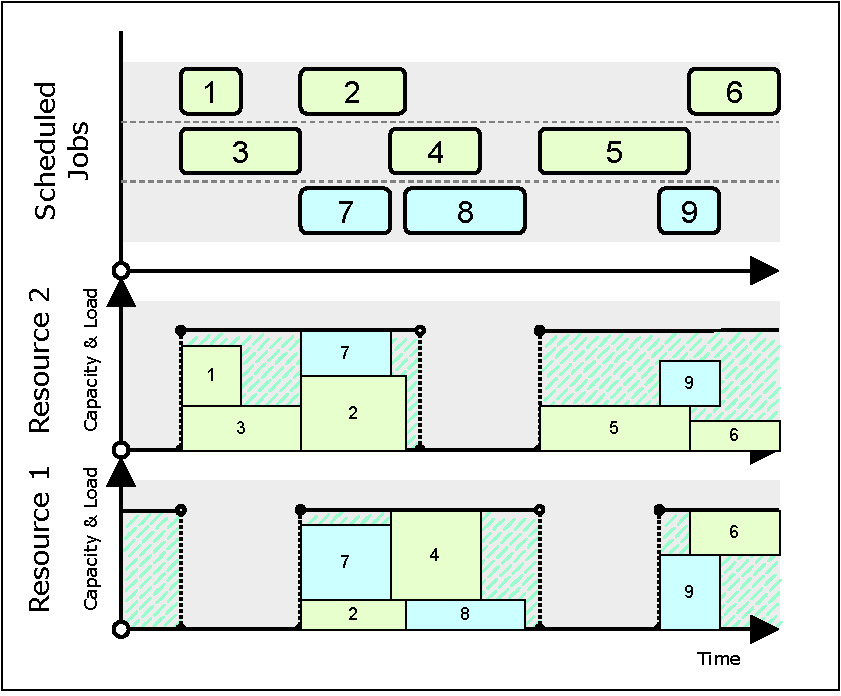
\includegraphics[width=\linewidth]{img/Schedule.pdf}
            Example of extended RCPSP schedule
        \end{center}
    \end{minipage}
}
% --------------------------------------------------------------------------------------------------------------------------
\leftalignedheaderbox{Goals}{name=goals, span=2, column=4, row=0,%
bottomaligned=problemStatement
}{
    \begin{itemize}[leftmargin=*]
        \item 
            Design a method for identifying bottlenecks in obtained schedules.
        
        \item
            Propose model constraint relaxations related to the bottleneck resources in the obtained schedules.
            Such relaxations should improve the tardiness of a specific target manufacturing order
            while not modifying the original schedule much.
            Additionally, the relaxations should correspond to feasible and practical real-world implementations.
    \end{itemize}
}
% ==========================================================================================================================
\leftalignedheaderbox{Identification Indicator-based Relaxing Algorithm}{%
name=iira,span=3,column=0,below=problemStatement,
% boxColorTwo=red!45!yellow!30
boxColorOne=\highlightcolorOne,
boxColorTwo=\highlightcolorTwo
}{
    We propose two \emph{bottleneck identification indicators} for the extended \acs{rcpsp}
    --- \acf{mrur} and \acf{auau}. Each computes a single numeric value for a given resource $k$.
    \vspace{-0.5em}
    \begin{align*}
        &\indMRUR{k} = \frac{\text{total consumption of $k$ by all jobs}}%
                           {\text{total capacity of $k$ over project makespan}}
        \\
        &\indAUAU{k} = \text{average utilization over uninterrupted active periods}\\[-2.2em]
        % \\
        % &\text{where utilization during active period} = \frac{\text{total active period consumption }}{\text{total active period capacity}}.
    \end{align*}
    % The \acf{iira} identifies a bottleneck resource using an identification indicator,
    % calculates a granular resource load functions for the bottleneck resource,
    % and determines the improvement potential of granular periods through convolution.
    % It the relaxes resource capacities of the bottleneck resource
    % during the granular period with highest computed improvement potential.
    % Finally, a solution to the modified problem is found
    % and proposed capacity changes are reduced to only include utilized changes.
    The \acf{iira} works as follows:
    \begin{center}
    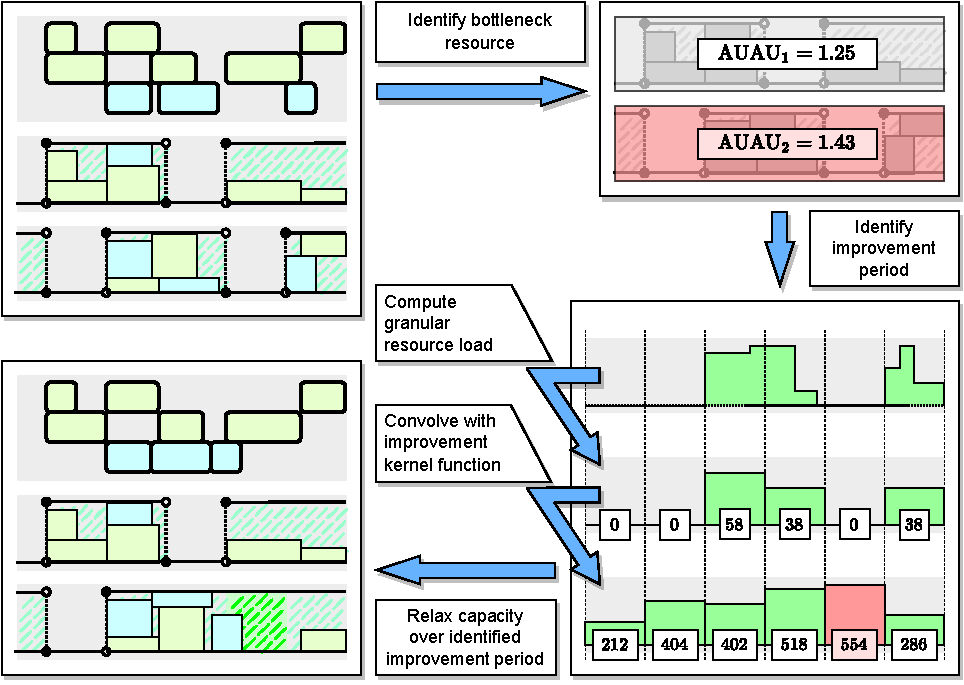
\includegraphics[width=\textwidth]{img/iira.pdf}
    \end{center}
    \vspace{-0.6em}
    The proposed resource capacity functions are reduced to only include utilized changes.
    The changes are then divided into \emph{migrations} and \emph{additions} based on available capacities
    on remaining resources.
}
% --------------------------------------------------------------------------------------------------------------------------
\leftalignedheaderbox{Schedule Suffix Interval Relaxing Algorithm}{%
name=ssira,span=3,column=3,below=problemStatement,
% boxColorTwo=red!45!yellow!30
boxColorOne=\highlightcolorOne,
boxColorTwo=\highlightcolorTwo
}{
    The \acf{ssira} relaxes \emph{suffixes of schedules} to obtain heuristic interval relaxation proposals.
    The algorithm focuses on the target manufacturing order
    by identifying improvement intervals only within its left-shift closure.
    The \emph{left-shift closure} of a manufacturing order is the set of jobs that,
    corresponding to various definitions, prevent the order from finishing earlier.
    \begin{center}
    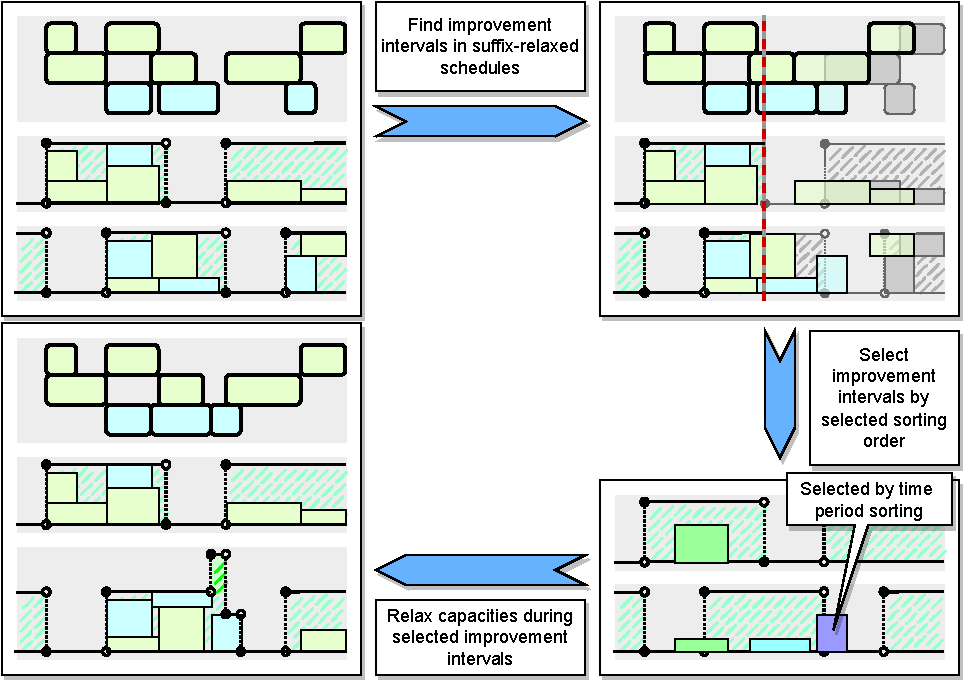
\includegraphics[width=\textwidth]{img/ssira.pdf}
    \end{center}
    \vspace{-0.6em}
    Same as in the \acs{iira}, the capacity changes are reduced and corresponding capacity \emph{migrations} and \emph{additions} are identified.
}
% ==========================================================================================================================
\leftalignedheaderbox{Experiments}{name=experiments, below=iira, span=3, row=0, column=0}{
    Numerical experiments we conducted to analyze the capabilities
    of the proposed methods. For that purpose, we designed a set of problem instances
    (based on PSPLIB instances) modeling the used extension of the RCPSP.

    We observed that the \highlight{SSIRA is more consistent in finding improving solutions} than the IIRA,
    while the \highlight{IIRA is able to find great improvements with low modification costs} on instances,
    where the SSIRA finds the same improvements with greater costs.
}		
% --------------------------------------------------------------------------------------------------------------------------
\leftalignedheaderbox{Summary}{name=summary, span=3, below=ssira, column=3, bottomaligned=experiments}{
    In this thesis, we
    \begin{itemize}[leftmargin=*]
        \item
            \highlight{designed the \acs{iira}} as a baseline solution adapting existing bottleneck identification approaches
            from the scheduling literature and proposing relaxations based on those identifications,\\[-1.8em]
        \item
            \highlight{designed the \acs{ssira}} as a novel approach to identifying schedule bottlenecks
            and relaxing related constraints in the \acs{rcpsp}, and\\[-1.8em]
        \item
            \highlight{conducted numerical experiments} showing that the \acs{iira} achieves great improvements for small costs,
            while the \acs{ssira} is more reliable in achieving improvements across various problem instances.
    \end{itemize}

    Future work could focus on modeling the relaxations as an optimization problem to obtain exact proposals
    capturing all model dependencies.
}
% Footer ===================================================================================================================
\headerbox{}{headershape=rectangle, name=repository, column=2, span=4, above=bottom, borderColor=maincolor,  boxheaderheight=1pt}{
    \begin{minipage}{.17\textwidth}
        \begin{center}
            % \vspace{-0.22cm}%
            \qrcode[height=2cm]{https://github.com/Krtiiik/RCPSPSandbox}%
        \end{center}
    \end{minipage}%
    \begin{minipage}{.66\textwidth}
        \textbf{\large\sffamily\color{maincolor}Project repository}
        \\[0.25em]
        \scriptsize\url{https://github.com/Krtiiik/RCPSPSandbox}
        % \vfill\hrule\vfill
        \vspace{0.55em}\hrule\vspace{0.55em}
        \hfill\textbf{\large\sffamily\color{maincolor}Bachelor thesis}
        \\[0.25em]
        \scriptsize\url{https://github.com/Krtiiik/Bottleneck-identification-for-constraint-relaxation-in-resource-constrained-project-scheduling/blob/main/thesis.pdf}
    \end{minipage}%
    \begin{minipage}{.17\textwidth}
        \begin{center}
            % \vspace{-0.22cm}%
            \qrcode[height=2cm]{https://github.com/Krtiiik/Bottleneck-identification-for-constraint-relaxation-in-resource-constrained-project-scheduling/blob/main/thesis.pdf}%
        \end{center}
    \end{minipage}%
}
\headerbox{}{headershape=rectangle, name=supervisor, column=0, span=2, above=bottom, borderColor=maincolor,  boxheaderheight=1pt, aligned=repository}{
    \textbf{\sffamily\large\color{maincolor}Supervisor}
    \\[0.4em]
    {\large RNDr. Jiří Švancara, Ph.D.}
    \\[0.1em]
    Department of Theoretical Computer Science and Mathematical Logic, MFF UK
}
\end{poster}
\end{document}
